%\documentclass[dvipdfmx]{beamer}      % platex の場合
\documentclass[handout]{beamer}        % lualatex の場合
\usepackage{mySld}
\usepackage{multicol}

\begin{document}
\title{基礎コンピュータ工学\\第5章 機械語プログラミング\\(パート4)}
\date{}

\begin{frame}
  \titlepage
  \centerline{\url{https://github.com/tctsigemura/TecTextBook}}
  \vfill
  \centerline{本スライドの入手:
    \raisebox{-7mm}{
\includegraphics[scale=0.3]{../Img/QRs5_4.png}}}
\end{frame}

%==============================================================================
%\begin{frame}
%  \frametitle
%  \tableofcontents
%\end{frame}

\section{ジャンプ命令}
%==============================================================================
\begin{frame}
  \frametitle{プログラムの流れ}
  \begin{itemize}
  \item プログラムは番地順に実行される(逐次実行).
  \item 実行が進んでいく流れを「プログラムの流れ」と呼ぶ.
  \item 「プログラムの流れ」はPCによって管理されている.
  \item 通常,PCは増加していく.
  \item 「プログラムの流れ」を別のアドレスに変えることも必要.
    \begin{itemize}
    \item 条件によって処理内容を変更したい場合.
    \item 同じ処理内容を繰り返したい場合.
    \end{itemize}
  \item 「プログラムの流れ」を変える命令を\textbf{ジャンプ命令}と呼ぶ. \\
    \textbf{「プログラムの流れ」を飛ばす = PCにアドレスをロードする}
  \end{itemize}
  \vfill
  \vfill
\end{frame}

%==============================================================================
\begin{frame}
  \frametitle{ジャンプ命令(7種類)}
  \begin{description}
  \item[無条件ジャンプ命令:]\emph{プログラムの流れ}を指定のアドレスに飛ばす.
  \item[条件ジャンプ命令:]条件が成立したときだけジャンプする.
  \end{description}
  \vfill

  \emph{無条件ジャンプ命令(JMP命令)の役割イメージ}\\
  {\ttfamily\small\begin{center}
    \begin{tabular}{|l|l|l|l l|} \hline
      番地 & 機械語 & ラベル & \multicolumn{2}{|c|}{ニーモニック} \\
      \hline
      00 & 10 08 &             & LD   & G0,08H                \\
      02 & 30 09 &             & ADD  & G0,09H                \\
      04 & 20 0A &             & ST   & G0,0AH                \\
      06 & A0 0B &             & JMP  & 0BH                   \\
      08 & 12    &             & \multicolumn{2}{|c|}{データ} \\
      09 & 34    &             & \multicolumn{2}{|c|}{データ} \\
      0A & 00    &             & \multicolumn{2}{|c|}{データ} \\
      0B & 30 09 &             & ADD  & G0,09H                \\
      0D & ...   &             & ...  &                       \\
      \hline
    \end{tabular}
    \end{center}}
  \vfill
\end{frame}

%==============================================================================
\begin{frame}
  \frametitle{JMP(Jump)命令(ニーモニックと命令フォーマット)}
  \begin{description}
  \item[無条件ジャンプ命令:]\emph{JMP(Jump)命令}
    \vfill

  \item[ニーモニック:]\texttt{JMP EA}~~~~~~~~~\texttt{(PC ← EA)}
    \vfill

  \item[命令フォーマット:] 2バイトの長さを持つ.\\
    \twoByte{$1010_2$}{$00_2$~\XR}{\A}
  \end{description}
  \vfill

  \emph{例:}メモリの$10_{16}$番地へ飛ぶ(ジャンプする).
  \begin{description}
  \item[ニーモニック:]\texttt{JMP 10H}~~~~~~~~~動作:

  \item[命令フォーマット:] 10Hを反映する.\\
    \twoByte{$1010_2$}{$00_2$~$00_2$}{$0001~0000_2$}
  \end{description}
  \vfill
\end{frame}

%==============================================================================
\begin{frame}
  \frametitle{JMP(Jump)命令(フローチャートとプログラム例)}
  \begin{description}
  \item[JMP命令のフローチャート:]  ←,→,↑,↓ など
    \vfill

  \item[フローチャートの例:]ADD命令を永遠に繰り返す.(無限ループ)\\
    \centerline{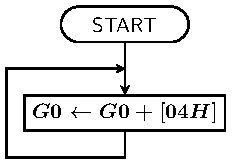
\includegraphics[scale=0.8]{../Tikz/flow0.pdf}}
    \vfill

  \item[プログラムの例:]0番地のADD命令を永遠に繰り返す.(無限ループ)\\
    {\ttfamily\small\begin{center}
      \begin{tabular}{|l|l|l|l l|} \hline
        番地 & 機械語 & ラベル & \multicolumn{2}{|c|}{ニーモニック} \\
        \hline
        00 & 30 04 & & ADD  & G0,04H \\
        02 & A0 00 & & JMP  & 00H \\
        \hline
      \end{tabular}
    \end{center}}
    \vfill

  \item[演習(1):]上のプログラムを4番地に1を格納した状態で実行する.\\
    STOPボタンでプログラムを停止しG0の値を確認する.
    \vfill
  \end{description}
\end{frame}

%==============================================================================
\begin{frame}
  \frametitle{ラベル}
  ニーモニックだけでプログラムを完結させるために使用する.
  \vfill
  \begin{itemize}
  \item JMP命令のプログラム例では,\\
    ジャンプ先のアドレスをニーモニックに中に数値で書いた.
  \vfill
  \item 機械語の番地が決まらないとニーモニックが完成しない.\\
    一方で,ニーモニックを書かないと機械語が完成しない.
  \vfill
  \item ニーモニックだけでプログラムを完結させる必要がある.\\
    →  場所(アドレス)に名前(ラベル)を付ける.
  \end{itemize}
  \vfill

  前のプログラムをラベルを使って書き直したもの.
  {\ttfamily\small\begin{center}
    \begin{tabular}{|l|l|l|l l|} \hline
      番地 & 機械語 & ラベル & \multicolumn{2}{|c|}{ニーモニック} \\
      \hline
      00 & 30 04 & \emph{LOOP} & ADD  & G0,04H      \\
      02 & A0 00 &             & JMP  & \emph{LOOP} \\
      \hline
    \end{tabular}\\
    \emph{LOOP} = 「輪」 ... 意味を持った名前を付けるとより良い.
  \end{center}}
  \vfill
\end{frame}

%==============================================================================
\begin{frame}
  \frametitle{DC(Define Constant)命令}
  まだ,データ部分がニーモニックで表現できていない.\\
%  ニーモニックでプログラムだけで完結させるためには,\\
  \vfill

  \begin{itemize}
  \item データもニーモニックで表現できる必要がある.
  \vfill

  \item DC命令はデータを記述するための疑似命令(≠機械語命令) \\
%  (ニーモニック中で「この行はデータですよ」と知らせる.)
  \vfill

  \item ニーモニック: \texttt{DC データの値}
  \vfill

  \item 前のプログラムを\emph{DC命令}を使って書き直したもの.
    {\ttfamily\footnotesize\begin{center}
      \begin{tabular}{|l|l|l|l l|} \hline
        番地 & 機械語 & ラベル & \multicolumn{2}{|c|}{ニーモニック} \\
        \hline
        00 & 30 04 & LOOP        & ADD        & G0,\emph{ONE} \\
        02 & A0 00 &             & JMP        & LOOP          \\
        04 & 01    & \emph{ONE}  & \emph{DC}  & \emph{1}      \\
        \hline
      \end{tabular}\\
      データの番地(04H)もラベル(ONE)で参照できる.
    \end{center}}
    \vfill

  \item フローチャートの例\\
    \centerline{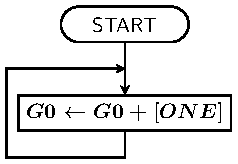
\includegraphics[scale=0.7]{../Tikz/flow0A.pdf}}
  \end{itemize}
  \vfill

 \end{frame}

%==============================================================================
\begin{frame}
  \frametitle{DS(Define Storage)命令}
  結果を格納する領域を作るための疑似命令.
  \begin{description}
  \item[ニーモニック:] \texttt{DS 領域の大きさ(バイト数)}
  \vfill

  \item[プログラムの例:]\emph{X番地}と\emph{Y番地}のデータの和を
    \emph{Z番地}に求める.\\
    (7番地と8番地のデータの和を9番地に求めると同じ)\\
    {\ttfamily\small\begin{center}
      \begin{tabular}{|l|l|l|l l|} \hline
        番地 & 機械語 & ラベル & \multicolumn{2}{|c|}{ニーモニック} \\
        \hline
        00 & 10 07 &          & LD        & G0,\emph{X}  \\
        02 & 30 08 &          & ADD       & G0,\emph{Y}  \\
        04 & 20 09 &          & ST        & G0,\emph{Z}  \\
        06 & FF    &          & HALT      &              \\
        07 & 12    & \emph{X} & \emph{DC} & \emph{12H}   \\
        08 & 34    & \emph{Y} & \emph{DC} & \emph{34H}   \\
        09 & 00    & \emph{Z} & \emph{DS} & \emph{1}     \\
        \hline
      \end{tabular}
    \end{center}}
    \vfill

    \item[DCとDSの区別:]プログラムの入力になるものをDCで準備する.\\
      プログラムの出力になるものをDSで場所を確保する.
  \end{description}
\end{frame}

%==============================================================================
\begin{frame}
  \frametitle{DC命令とDS命令の使い分け}
  入力となるデータを色々変化させたい場合.
  \begin{description}
  \item[プログラムの例:]
    X番地のデータに\emph{1を}加えたものをZ番地に求める.\\
    {\ttfamily\small\begin{center}
      \begin{tabular}{|l|l|l|l l|} \hline
        番地 & 機械語 & ラベル & \multicolumn{2}{|c|}{ニーモニック} \\
        \hline
        00 & 10 08 &            & LD        & G0,X          \\
        02 & 30 07 &            & ADD       & G0,\emph{ONE} \\
        04 & 20 09 &            & ST        & G0,Z          \\
        06 & FF    &            & HALT      &               \\
        07 & 01    & \emph{ONE} & \emph{DC} & \emph{1}      \\
        08 & 00    & \emph{X}   & \emph{DS} & \emph{1}      \\
        09 & 00    & Z          & DS        & 1             \\
        \hline
      \end{tabular}
    \end{center}}
    \vfill

    \item[DCとDSの区別:]値が変化しないものをDCで準備する.\\
      入力になるものは,典型的な値をDCで準備する.\\
      入力になるものは,後で決めるのでDSで場所を確保する.\\
      出力は,DSで場所を確保する.
  \end{description}
\end{frame}

%==============================================================================
\begin{frame}
  \frametitle{まとめ}
  \emph{学んだこと}
  \begin{itemize}
  \item 無条件ジャンプ命令(JMP命令)
  \item ラベル
  \item データを表現する命令(DC命令)
  \item データ領域を予約する命令(DS命令)
%  \item DC命令とDS命令の使い分け
  \end{itemize}
  \vfill

  \emph{演習(2)}(以下の目的で演習を行う)
  \begin{enumerate}
  \item[1.] PCの役割を再確認する.
  \item[2.] PCとJMP命令の関係を調べる.
  \item[3.] 計算結果とフラグの関係を調べる.※
  \item[4.] ステップモード実行の練習をする.
  \item[5.] ブレークモード実行の練習をする.
  \end{enumerate}
  \vfill
  ※次回はフラグの値を条件にするジャンプ命令を学ぶ.
  \vfill
\end{frame}

%==============================================================================
%\begin{frame}
%  \frametitle{}
%\end{frame}

\end{document}
